\ifx\wholebook\relax \else

\documentclass[UTF8]{article}
\usepackage[nomarginpar
  %, margin=.5in
]{geometry}

\addtolength{\oddsidemargin}{-0.05in}
\addtolength{\evensidemargin}{-0.05in}
\addtolength{\textwidth}{0.1in}

\usepackage[cn]{../../prelude}

\setcounter{page}{1}

\begin{document}

\title{前言}

\author{刘新宇
\thanks{{\bfseries 刘新宇} \newline
  Email: liuxinyu95@gmail.com \newline}
  }

\maketitle
\fi

\markboth{前言}{编程中的数学}

%\frontmatter{前言}
\chapter*{前言}
%\phantomsection  % so hyperref creates bookmarks
%\addcontentsline{toc}{chapter}{前言}

我讲一个从马爷爷那里听来的故事。有一年春节的时候,北京地坛公园的庙会热闹非凡、里里外外人山人海,小朋友们拿着压岁钱在各种摊位上买自己喜欢的玩具。公园外路边有一个摊位上围了一群人。地上一字排开摆了九个小玩具,每个玩具上依次贴着一元、二元、三元……直到九元的标签。摊主一边向大家吆喝,一边讲解游戏规则:“大家快来玩套圈游戏!一次一元钱,你扔一个,我扔一个,一个玩具只能套一个圈。谁能先套中三个加在一起值十五元的玩具算谁赢,你要是赢了,所有套中的玩具都归你。”

\vspace{5mm}
\begin{adjustbox}{max width=\textwidth}
\begin{tabular}{|c|c|c|c|c|c|c|c|c|}
\hline
中国结 & 风车 & 不倒翁 & 孙悟空面具 & 小猪存钱罐 & 九连环 & 汽车 & 兔爷 & 走马灯 \\
\hline
1 & 2 & 3 & 4 & 5 & 6 & 7 & 8 & 9 \\
\hline
\end{tabular}
\end{adjustbox}
\vspace{5mm}

有个小男孩掏出一元钱,拿了一个红色的圈,使劲一扔。真准!正好套在了七块钱的玩具汽车上,摊主拿出一个蓝色的圈,一下子套中了八块钱的兔爷。

\vspace{5mm}
\begin{adjustbox}{max width=\textwidth}
\begin{tabular}{|c|c|c|c|c|c|c|c|c|}
\hline
中国结 & 风车 & 不倒翁 & 孙悟空面具 & 小猪存钱罐 & 九连环 & 汽车 & 兔爷 & 走马灯 \\
\hline
1 & 2 & 3 & 4 & 5 & 6 & 7 & 8 & 9 \\
\hline
  &   &   &   &   &   & 男孩 & 摊主 & \\
\hline
\end{tabular}
\end{adjustbox}
\vspace{5mm}

小男孩又花了一元钱,这次他套中了价值两元的一个风车,这样只要他下次再套中那个六元的九连环就赢了。可这次摊主不慌不忙地套住了那只九连环。

\vspace{5mm}
\begin{adjustbox}{max width=\textwidth}
\begin{tabular}{|c|c|c|c|c|c|c|c|c|}
\hline
中国结 & 风车 & 不倒翁 & 孙悟空面具 & 小猪存钱罐 & 九连环 & 汽车 & 兔爷 & 走马灯 \\
\hline
1 & 2 & 3 & 4 & 5 & 6 & 7 & 8 & 9 \\
\hline
  & 男孩  &   &   &   & 摊主  & 男孩 & 摊主 & \\
\hline
\end{tabular}
\end{adjustbox}
\vspace{5mm}

这下可糟了,如果接下来摊主再套中那个一元钱的中国结,小男孩就要输了。小男孩涨红了脸,只能抢先去套那个中国结,他试了两次终于套中了。

\vspace{5mm}
\begin{adjustbox}{max width=\textwidth}

\begin{tabular}{|c|c|c|c|c|c|c|c|c|}
\hline
中国结 & 风车 & 不倒翁 & 孙悟空面具 & 小猪存钱罐 & 九连环 & 汽车 & 兔爷 & 走马灯 \\
\hline
1 & 2 & 3 & 4 & 5 & 6 & 7 & 8 & 9 \\
\hline
男孩  & 男孩  &   &   &   & 摊主  & 男孩 & 摊主 & \\
\hline
\end{tabular}
\end{adjustbox}
\vspace{5mm}

摊主接下来扔了一个圈,套住了四元钱的孙悟空面具。小男孩套住了五元钱的小猪存钱罐。

\vspace{5mm}
\begin{adjustbox}{max width=\textwidth}
\begin{tabular}{|c|c|c|c|c|c|c|c|c|}
\hline
中国结 & 风车 & 不倒翁 & 孙悟空面具 & 小猪存钱罐 & 九连环 & 汽车 & 兔爷 & 走马灯 \\
\hline
1 & 2 & 3 & 4 & 5 & 6 & 7 & 8 & 9 \\
\hline
男孩  & 男孩  &   & 摊主  & 男孩  & 摊主  & 男孩 & 摊主 & \\
\hline
\end{tabular}
\end{adjustbox}
\vspace{5mm}

但是摊主扔出一个圈,套住了三元的不倒翁。由于3 + 4 + 8 = 15,小男孩输了。

\vspace{5mm}
\begin{adjustbox}{max width=\textwidth}

\begin{tabular}{|c|c|c|c|c|c|c|c|c|}
\hline
中国结 & 风车 & 不倒翁 & 孙悟空面具 & 小猪存钱罐 & 九连环 & 汽车 & 兔爷 & 走马灯 \\
\hline
1 & 2 & 3 & 4 & 5 & 6 & 7 & 8 & 9 \\
\hline
男孩  & 男孩  & 摊主  & 摊主  & 男孩  & 摊主  & 男孩 & 摊主 & \\
\hline
\end{tabular}
\end{adjustbox}
\vspace{5mm}

周围的人看着很好玩,也纷纷掏钱套圈玩。马爷爷看了一阵,觉得很奇怪,大多数情况下都是摊主赢,偶尔会平局。马爷爷怀疑摊主一定有什么秘密,他只是为了避免人们怀疑,有时才故意输掉游戏。

马爷爷回到家,电视里正在讲中国古老的《河图洛书》,据说在文字尚未发明之前,伏羲治理天下的时候,在黄河支流,有乌龟背负着神秘的图案爬上岸来。如果把图案中的圆点数目用现代的方法表示出来,就是一个数学上的三阶幻方。

\begin{figure}[htbp]
 \centering
 \subcaptionbox{洛书}[0.45\linewidth]{ 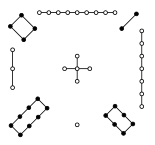
\includegraphics[scale=0.6]{img/luo-shu.png}}
 \subcaptionbox{三阶幻方}[0.45\linewidth]{
   \begin{tabular}{|c|c|c|}
   \hline
   4 & 9 & 2 \\
   \hline
   3 & 5 & 7 \\
   \hline
   8 & 1 & 6 \\
   \hline
   \end{tabular}
   \vspace{8mm}
 }
 \captionsetup{labelformat=empty}
 \caption{}
 \label{fig:luo-shu}
\end{figure}

% 考虑一一映射反向的情况。
可别被这个名字吓到,就是方形的九个格子里每行、每列、两个对角线上的三个数字加起来都相等,都等于十五。例如第一行的数字相加是4 + 9 + 2 = 15,第三列的数字相加是2 + 7 + 6 = 15,左上右下的对角线的数字相加是4 + 5 + 6 = 15。等一等——马爷爷想,我现在知道庙会里套圈游戏背后的秘密了。如果要套中的三个玩具加起来等于十五元,那么就相当于套中了幻方的一行、一列、或一个对角线。如果摊主在柜台里偷偷藏一张三阶幻方的图,那么他实际上相当于在和游人玩俗称“一条龙”的井字棋游戏。

\begin{figure}[htbp]
 \centering
 \subcaptionbox{三阶幻方}[0.45\linewidth]{
   \begin{tabular}{|c|c|c|}
   \hline
   4 & 9 & 2 \\
   \hline
   3 & 5 & 7 \\
   \hline
   8 & 1 & 6 \\
   \hline
   \end{tabular}
   \vspace{3mm}
 }
 \subcaptionbox{井字棋游戏}[0.45\linewidth]{
   \begin{tabular}{c|c|c}
   $\times$ &  & $\bigcirc$ \\
   \hline
   $\times$ & $\times$ &  \\
   \hline
   $\bigcirc$ & $\times$ & $\bigcirc$ \\
   \end{tabular}
   \vspace{3mm}
 }
 \captionsetup{labelformat=empty}
 \caption{}
 \label{fig:bingo-magic-square}
\end{figure}

庙会中那个小男孩和摊主的套圈游戏相当于下面的井字棋对局。摊主在关键的第三步中给小男孩设置了一个陷阱,他在第一列上和一个对角线上同时可能连成直线,如果小男孩套中3,则摊主套中5依然能赢。如果了解过博弈游戏,或者知道一点编程,你就知道井字棋游戏没有必胜的策略,如果游戏双方都足够小心,结果一定是平局。偷偷拥有三阶幻方图的摊主这样就站在了不败的地位上,而其他游客一无所知。

\begin{figure}[htbp]
 \centering
 \subcaptionbox{三阶幻方}[0.45\linewidth]{
   \begin{tabular}{|c|c|c|}
   \hline
   4 & 9 & 2 \\
   \hline
   3 & 5 & 7 \\
   \hline
   8 & 1 & 6 \\
   \hline
   \end{tabular}
   \vspace{3mm}
 }
 \subcaptionbox{第一步,男孩套中7,摊主套中8}[0.45\linewidth]{
   \begin{tabular}{c|c|c}
   &  & \\
   \hline
   &  & $\times$ \\
   \hline
   $\bigcirc$ & & \\
   \end{tabular}
   \vspace{3mm}
 } \vspace{3mm} \\
 \subcaptionbox{第二步,男孩套中2,摊主套中6}[0.45\linewidth]{
   \begin{tabular}{c|c|c}
   &  & $\times$\\
   \hline
   &  & $\times$ \\
   \hline
   $\bigcirc$ & & $\bigcirc$ \\
   \end{tabular}
   \vspace{3mm}
 }
 \subcaptionbox{第三步,男孩套中1,摊主套中4}[0.45\linewidth]{
   \begin{tabular}{c|c|c}
   $\bigcirc$ &  & $\times$\\
   \hline
   &  & $\times$ \\
   \hline
   $\bigcirc$ & $\times$ & $\bigcirc$ \\
   \end{tabular}
   \vspace{3mm}
 } \vspace{3mm} \\
 \subcaptionbox{第四步,男孩套中5,摊主套中3,摊主胜}[0.45\linewidth]{
   \begin{tabular}{c|c|c}
   $\pmb{\bigcirc}$ &  & $\times$\\
   \hline
   $\pmb{\bigcirc}$ &  $\times$ & $\times$ \\
   \hline
   $\pmb{\bigcirc}$ & $\times$ & $\bigcirc$ \\
   \end{tabular}
   \vspace{3mm}
 }
 \captionsetup{labelformat=empty}
 \caption{}
 \label{fig:game-steps}
\end{figure}

这个故事是真的么?当然不是,马爷爷是个虚构的人物,他在真实世界中名叫马丁$\cdot$加德纳——举世闻名的美国趣味数学大师。这个故事来自他的《啊哈!灵机一动》。故事不是发生在北京的地坛公园,而是美国的乡村小镇。摊主名叫卡内,而玩游戏的小男孩实际是一位女士。这个游戏也不是中国传统的套圈游戏,而是用硬币盖住一排数字。

这个故事和其中所讲的游戏不断在说着一个重要的概念——同构。庙会上的套圈游戏和井字棋同构,一行九个数字对应三行三列的格子,相加等于15的目标对应九宫格中的行、列、对角线,古老的《洛书》对应数学幻方,马爷爷对应加德纳,中国的春节庙会对应美国乡村游乐……这其实也是本书想传达的概念,编程和数学同构,和艺术同构,和音乐同构。伟大的发现背后有曲折的故事和性格迥异的数学家。

这个故事还有一层隐喻,问题的表象下隐藏着和它同构的理论实质,我们需要了解抽象的本质而不被具体的现象蒙住眼睛。在人工智能和机器学习日新月异的今天,我们能否还靠着一点点聪明和工程实践继续前行?我们是否要打开那些神秘的黑盒子找到那个指引我们前进的地图?

\vspace{15mm}

刘新宇

二零一九年五月于北京

\begin{Exercise}
\Question{编程实现一个井字棋游戏是传统人工智能中的经典问题,而计算机可以轻松算出三个数字的和并判断其是否等于15。请利用这个同构编写一个简化的井字棋程序,并做到不被人类玩家击败\footnote{本书附录提供了全部习题的答案,希望读者先自行思考再参考后面的答案。}。}
\end{Exercise}

\vspace{10mm}

本书的电子版可以在\url{https://github.com/liuxinyu95/unplugged}下载。如果希望获得纸质版,请联系作者:liuxinyu95@gmail.com

\ifx\wholebook\relax \else

\expandafter\enddocument
%\end{document}

\fi
